\documentclass[times, utf8, seminar]{fer}

\usepackage[hidelinks]{hyperref}
\usepackage{subfig}
\usepackage{float}

\begin{document}

\title{6. Domaća zadaća - Sustav ANFIS \engl{Adaptive Neuro-Fuzzy Inference System}}
\author{0036506587 Darijo Brčina}

\maketitle

\tableofcontents

\chapter{Zadatak 1}
Funkcija pogreške za \textit{k}-ti uzorak:
\[E_k = \frac{1}{2}(y_k-o_k)^2,\]
gdje \textit{y\textsubscript{k}} predstavlja željeni izlaz za \textit{k}-ti uzorak, dok \textit{o\textsubscript{k}} predstavlja stvarni izlaz neuro-fuzzy sustava.


Ažuriranje parametara u skladu s algoritmom gradijentnog spusta:
\[\psi(t+1) = \psi(t) - \eta \cdot \frac{\partial E_k}{\partial \psi}.\]

Promatrat ćemo ANFIS koji koristi zaključivanje tipa 3 (metodu Takagi-Sugeno-Kang). Neuro-fuzzy sustav će imati dva ulaza i jedan izlaz čime će obavljati preslikavanje $\mathbb{R}^2 \rightarrow \mathbb{R}$. U općem slučaju, neuro-fuzzy sustav će raspolagati s \textit{m} pravila:
\begin{itemize}
    \item[] $\mathbb{R}_1 : \text{Ako } x \text{ je } A_1 \text{ i } y \text{ je } B_1 \text{ tada } z = p_1x + q_1y + r_1$
    \item[] $\mathbb{R}_2 : \text{Ako } x \text{ je } A_2 \text{ i } y \text{ je } B_2 \text{ tada } z = p_2x + q_2y + r_2$
    \item[] $\dots$
    \item[] $\mathbb{R}_m : \text{Ako } x \text{ je } A_m \text{ i } y \text{ je } B_m \text{ tada } z = p_mx + q_my + r_m$
\end{itemize}
Uz zadani skup pravila od \textit{m} pravila, temeljem primjera za učenje sustav treba naučiti ukupno $2 \cdot m$ neizrazitih skupova koji se nalaze u antecedent dijelu pravila i $3 \cdot m$ parametara koji određuju \textit{m} funkcija u konzekvens dijelovima pravila.

Neizraziti skupovi \textit{A} i \textit{B} su definirani sljedećim funkcijama pripadnosti:
\[\alpha_i = A_i(x) = \frac{1}{1 + e^{b_i(x-a_i)}},\]
\[\beta_i = B_i(y) = \frac{1}{1 + e^{d_i(y-c_i)}}.\]


Iz navedenog se može zaključiti da je potrebno naučiti sveukupno $7 \cdot m$ parametara sustava.

Stvarni izlaz neuro-fuzzy sustava je definiran na sljedeći način:
\[o_k = \frac{\sum_{i=1}^{m} \pi_iz_i}{\sum_{i=1}^{m} \pi_i},\]
gdje je $\pi_i = \alpha_i \cdot \beta_i$. Sada kada znamo kako je sve definirano, možemo izvesti formule za ažuriranje svih parametara tijekom učenja algoritmom gradijenti spust, pa krenimo:
\begin{enumerate}
    \item 
        \[\frac{\partial E_k}{\partial a_i} = \frac{\partial E_k}{\partial o_k} \frac{\partial o_k}{\partial \pi_i}     \frac{\partial \pi_i}{\partial \alpha_i} \frac{\partial \alpha_i}{\partial a_i}\]
        \[\frac{\partial E_k}{\partial o_k} = \frac{\partial}{\partial o_k}(\frac{1}{2}(y_k-o_k)^2) = 2 \cdot \frac{1}{2}(y_k-o_k) \cdot (-1) = -(y_k-o_k)\]
        \[\frac{\partial o_k}{\partial \pi_i} = \frac{\partial}{\partial \pi_i}(\frac{\sum_{j=1}^{m} \pi_jz_j}{\sum_{j=1}^{m} \pi_j}) = \frac{z_i \sum_{j=1,j \neq i}^{m} \pi_j - \sum_{j=1,j \neq i}^{m} \pi_jz_j \cdot 1}{(\sum_{j=1}^{m} \pi_j)^2} = \frac{\sum_{j=1,j \neq i}^{m} \pi_j(z_i-z_j)}{(\sum_{j=1}^{m} \pi_j)^2}\]
        \[\frac{\partial \pi_i}{\partial \alpha_i} = \frac{\partial}{\partial \alpha_i}(\alpha_i \cdot \beta_i) = \beta_i\]
        \[\frac{\partial \alpha_i}{\partial a_i} = \frac{\partial}{\partial a_i}(\frac{1}{1 + e^{b_i(x-a_i)}}) = (-1) \cdot \frac{1}{(1 + e^{b_i(x-a_i)})^2} \cdot e^{b_i(x-a_i)} \cdot (-b_i) = \alpha_i(1-\alpha_i) \cdot b_i\]
        \[\frac{\partial E_k}{\partial a_i} = -(y_k-o_k)\frac{\sum_{j=1,j \neq i}^{m} \pi_j(z_i-z_j)}{(\sum_{j=1}^{m} \pi_j)^2}\beta_i\alpha_i(1-\alpha_i)b_i\]
        \[\Longrightarrow a_i(t+1) = a_i(t) + \eta \cdot (y_k-o_k)\frac{\sum_{j=1,j \neq i}^{m} \pi_j(z_i-z_j)}{(\sum_{j=1}^{m} \pi_j)^2}\beta_i\alpha_i(1-\alpha_i)b_i\]
    \item 
        \[\frac{\partial E_k}{\partial b_i} = \frac{\partial E_k}{\partial o_k} \frac{\partial o_k}{\partial \pi_i}     \frac{\partial \pi_i}{\partial \alpha_i} \frac{\partial \alpha_i}{\partial b_i}\]
        \[\frac{\partial E_k}{\partial o_k} = -(y_k-o_k)\]
        \[\frac{\partial o_k}{\partial \pi_i} = \frac{\sum_{j=1,j \neq i}^{m} \pi_j(z_i-z_j)}{(\sum_{j=1}^{m} \pi_j)^2}\]
        \[\frac{\partial \pi_i}{\partial \alpha_i} = \beta_i\]
        \[\frac{\partial \alpha_i}{\partial b_i} = \frac{\partial}{\partial b_i}(\frac{1}{1 + e^{b_i(x-a_i)}}) = (-1) \cdot \frac{1}{(1 + e^{b_i(x-a_i)})^2} \cdot e^{b_i(x-a_i)} \cdot (x-a_i) = \alpha_i(1-\alpha_i) \cdot (a_i-x)\]
        \[\frac{\partial E_k}{\partial b_i} = -(y_k-o_k)\frac{\sum_{j=1,j \neq i}^{m} \pi_j(z_i-z_j)}{(\sum_{j=1}^{m} \pi_j)^2}\beta_i\alpha_i(1-\alpha_i)(a_i-x)\]
        \[\Longrightarrow b_i(t+1) = b_i(t) + \eta \cdot (y_k-o_k)\frac{\sum_{j=1,j \neq i}^{m} \pi_j(z_i-z_j)}{(\sum_{j=1}^{m} \pi_j)^2}\beta_i\alpha_i(1-\alpha_i)(a_i-x)\]
    \item Po uzoru na ažuriranje parametra \textit{a} uz $\frac{\partial \pi_i}{\partial \beta_i} = \alpha_i$:
        \[\Longrightarrow c_i(t+1) = c_i(t) + \eta \cdot (y_k-o_k)\frac{\sum_{j=1,j \neq i}^{m} \pi_j(z_i-z_j)}{(\sum_{j=1}^{m} \pi_j)^2}\alpha_i\beta_i(1-\beta_i)d_i\]
    \item Po uzoru na ažuriranje parametra \textit{b} uz $\frac{\partial \pi_i}{\partial \beta_i} = \alpha_i$:
        \[\Longrightarrow d_i(t+1) = d_i(t) + \eta \cdot (y_k-o_k)\frac{\sum_{j=1,j \neq i}^{m} \pi_j(z_i-z_j)}{(\sum_{j=1}^{m} \pi_j)^2}\alpha_i\beta_i(1-\beta_i)(c_i-y)\]
    \item
         \[\frac{\partial E_k}{\partial p_i} = \frac{\partial E_k}{\partial o_k} \frac{\partial o_k}{\partial p_i}\]
         \[\frac{\partial E_k}{\partial o_k} = -(y_k-o_k)\]
         \[\frac{\partial o_k}{\partial p_i} = \frac{\partial}{\partial p_i}(\frac{\sum_{j=1}^{m} \pi_jz_j}{\sum_{j=1}^{m} \pi_j}) = \frac{\partial}{\partial p_i}(\frac{\sum_{j=1}^{m} \pi_j(p_jx + q_jy + r_j)}{\sum_{j=1}^{m} \pi_j}) = \frac{\pi_i}{\sum_{j=1}^{m} \pi_j}x\]
         \[\frac{\partial E_k}{\partial p_i} = -(y_k-o_k)\frac{\pi_i}{\sum_{j=1}^{m} \pi_j}x\]
         \[\Longrightarrow p_i(t+1) = p_i(t) + \eta \cdot (y_k-o_k)\frac{\pi_i}{\sum_{j=1}^{m} \pi_j}x\]
    \item
         \[\frac{\partial E_k}{\partial q_i} = \frac{\partial E_k}{\partial o_k} \frac{\partial o_k}{\partial q_i}\]
         \[\frac{\partial E_k}{\partial o_k} = -(y_k-o_k)\]
         \[\frac{\partial o_k}{\partial q_i} = \frac{\partial}{\partial q_i}(\frac{\sum_{j=1}^{m} \pi_jz_j}{\sum_{j=1}^{m} \pi_j}) = \frac{\partial}{\partial q_i}(\frac{\sum_{j=1}^{m} \pi_j(p_jx + q_jy + r_j)}{\sum_{j=1}^{m} \pi_j}) = \frac{\pi_i}{\sum_{j=1}^{m} \pi_j}y\]
         \[\frac{\partial E_k}{\partial q_i} = -(y_k-o_k)\frac{\pi_i}{\sum_{j=1}^{m} \pi_j}y\]
         \[\Longrightarrow q_i(t+1) = q_i(t) + \eta \cdot (y_k-o_k)\frac{\pi_i}{\sum_{j=1}^{m} \pi_j}y\]
    \item
         \[\frac{\partial E_k}{\partial r_i} = \frac{\partial E_k}{\partial o_k} \frac{\partial o_k}{\partial r_i}\]
         \[\frac{\partial E_k}{\partial o_k} = -(y_k-o_k)\]
         \[\frac{\partial o_k}{\partial r_i} = \frac{\partial}{\partial r_i}(\frac{\sum_{j=1}^{m} \pi_jz_j}{\sum_{j=1}^{m} \pi_j}) = \frac{\partial}{\partial q_i}(\frac{\sum_{j=1}^{m} \pi_j(p_jx + q_jy + r_j)}{\sum_{j=1}^{m} \pi_j}) = \frac{\pi_i}{\sum_{j=1}^{m} \pi_j}\]
         \[\frac{\partial E_k}{\partial r_i} = -(y_k-o_k)\frac{\pi_i}{\sum_{j=1}^{m} \pi_j}\]
         \[\Longrightarrow r_i(t+1) = r_i(t) + \eta \cdot (y_k-o_k)\frac{\pi_i}{\sum_{j=1}^{m} \pi_j}\]
\end{enumerate}
\textbf{Napomena:} Ažuriranje parametara je izvedeno za \textit{online} tip učenja, dok bi se za pravi gradijent morala uzimati suma pogrešaka svih uzoraka za učenje tijekom pronalaska parcijalnih derivacija, tj.
\[E = \sum_{k=1}^{N} E_k.\]

\chapter{Zadatak 3}

\begin{figure}[H]
    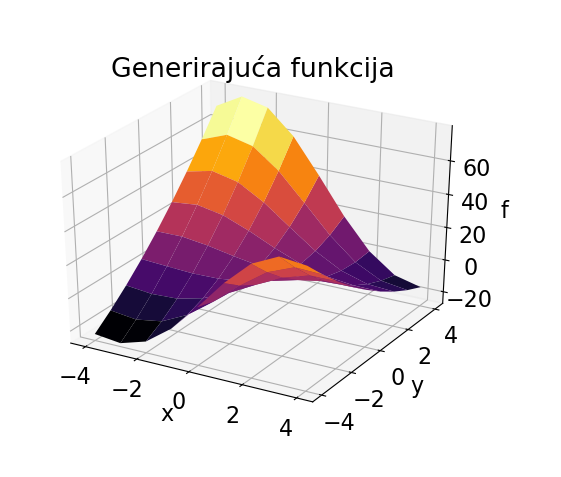
\includegraphics[scale=0.9]{img/generirajuca.png}
    \caption{Graf generirajuće funkcije}
\end{figure}

\chapter{Zadatak 4}

\section{Jedno pravilo}
\begin{figure}[H]
    \subfloat{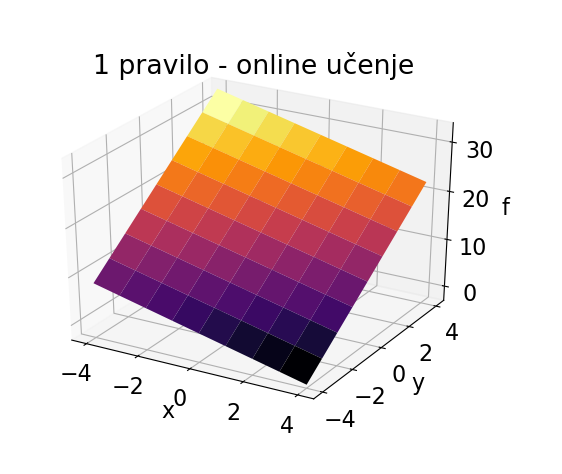
\includegraphics[width=0.5\textwidth]{img/anfis-funkcija-jedno-pravilo-online.png}}
    \subfloat{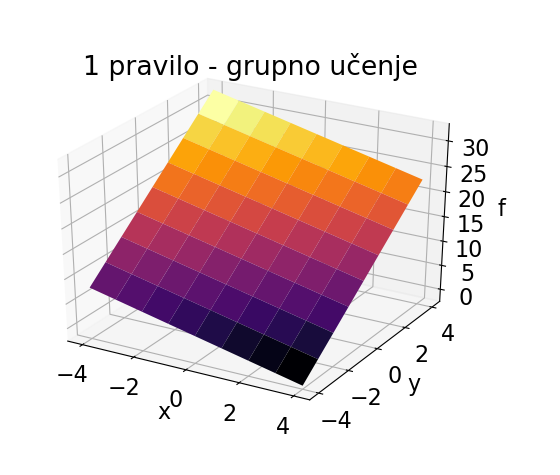
\includegraphics[width=0.5\textwidth]{img/anfis-funkcija-jedno-pravilo-grupno.png}}
    \caption{Grafovi aproksimirane generirajuće funkcije}
\end{figure}
\begin{figure}[H]
    \subfloat{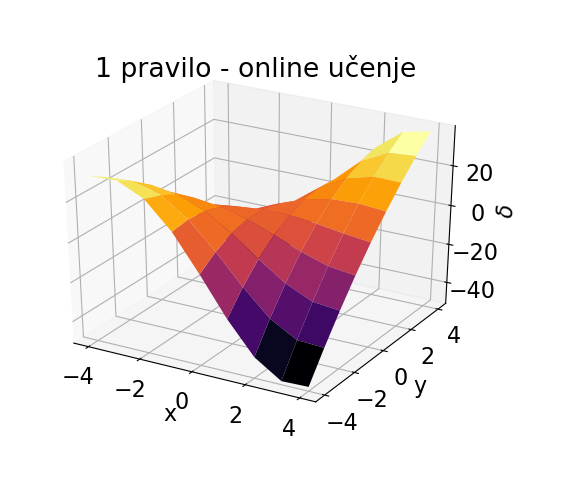
\includegraphics[width=0.5\textwidth]{img/delta-jedno-pravilo-online.png}}
    \subfloat{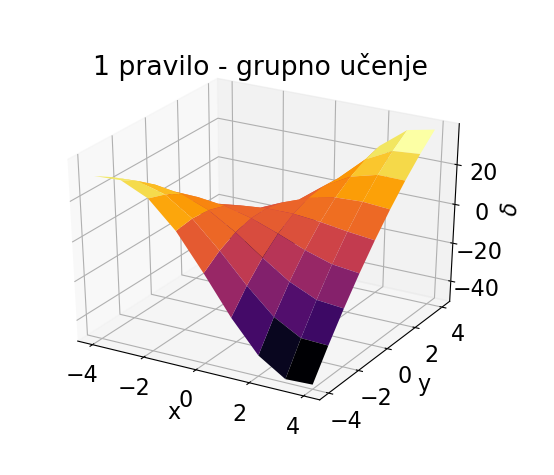
\includegraphics[width=0.5\textwidth]{img/delta-jedno-pravilo-grupno.png}}
    \caption{Grafovi pogrešaka}
\end{figure}

\section{Dva pravila}
\begin{figure}[H]
    \subfloat{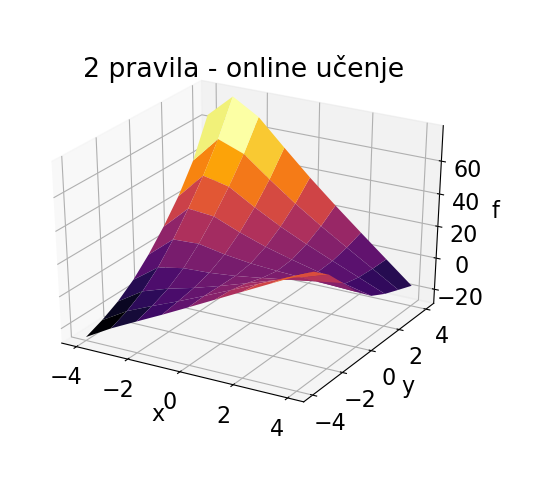
\includegraphics[width=0.5\textwidth]{img/anfis-funkcija-dva-pravila-online.png}}
    \subfloat{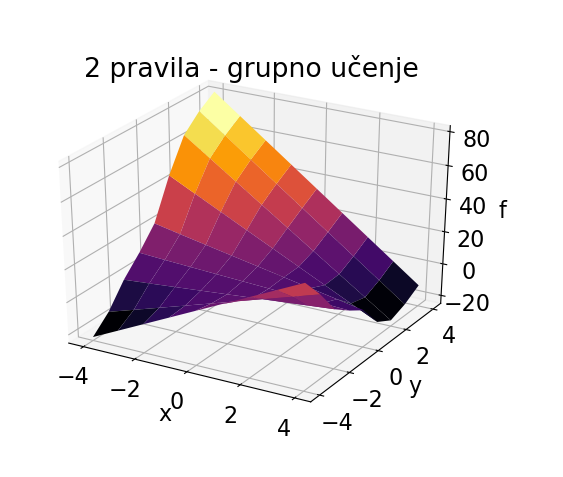
\includegraphics[width=0.5\textwidth]{img/anfis-funkcija-dva-pravila-grupno.png}}
    \caption{Grafovi aproksimirane generirajuće funkcije}
\end{figure}
\begin{figure}[H]
    \subfloat{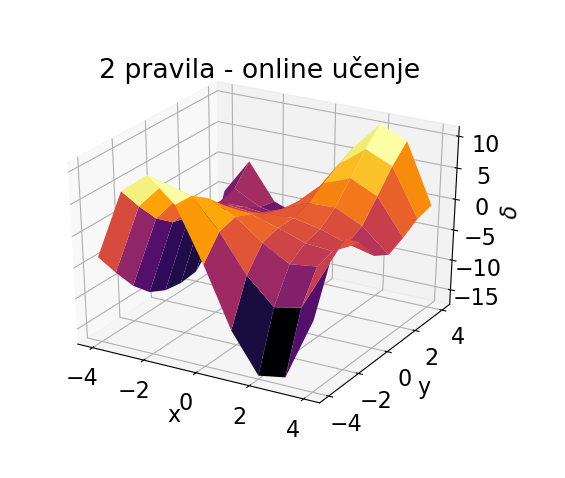
\includegraphics[width=0.5\textwidth]{img/delta-dva-pravila-online.png}}
    \subfloat{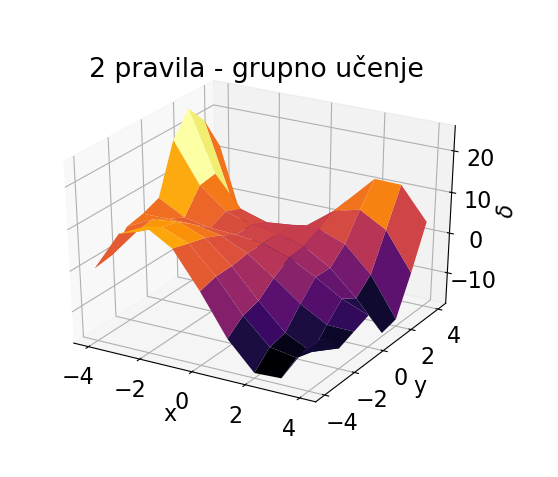
\includegraphics[width=0.5\textwidth]{img/delta-dva-pravila-grupno.png}}
    \caption{Grafovi pogrešaka}
\end{figure}

\section{Prikladan broj pravila - sedam}
\begin{figure}[H]
    \subfloat{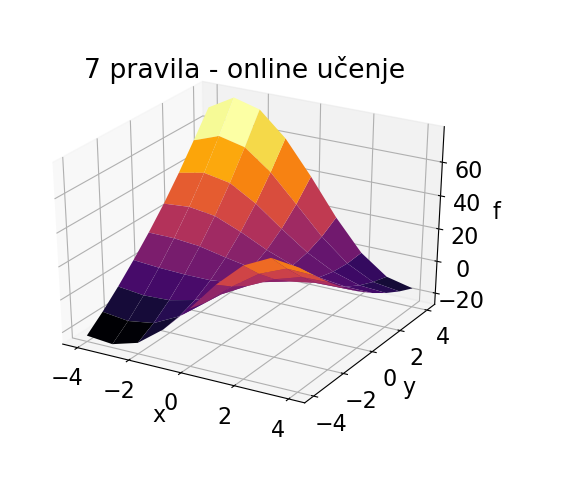
\includegraphics[width=0.5\textwidth]{img/anfis-funkcija-sedam-pravila-online.png}}
    \subfloat{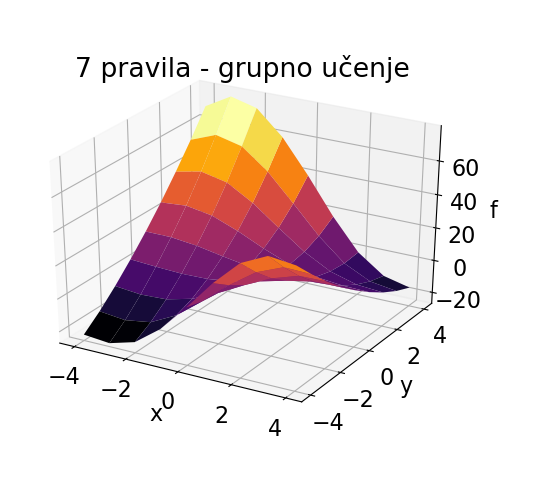
\includegraphics[width=0.5\textwidth]{img/anfis-funkcija-sedam-pravila-grupno.png}}
    \caption{Grafovi aproksimirane generirajuće funkcije}
\end{figure}
\begin{figure}[H]
    \subfloat{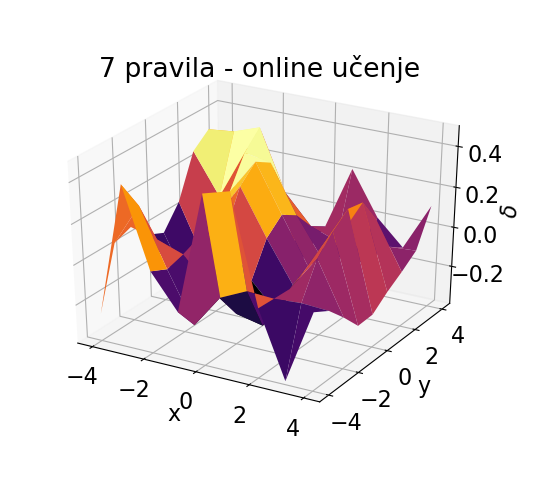
\includegraphics[width=0.5\textwidth]{img/delta-sedam-pravila-online.png}}
    \subfloat{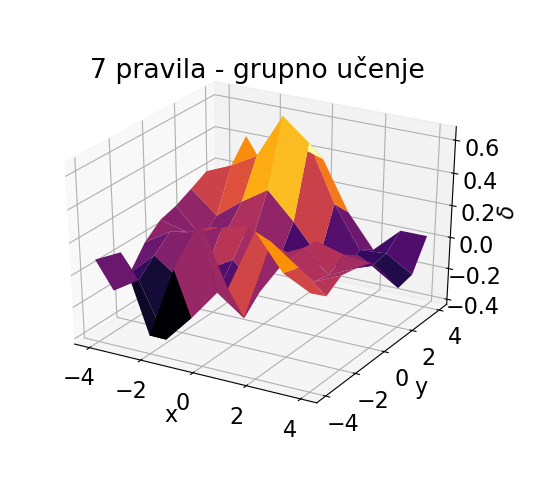
\includegraphics[width=0.5\textwidth]{img/delta-sedam-pravila-grupno.png}}
    \caption{Grafovi pogrešaka}
\end{figure}

\chapter{Zadatak 5}
\begin{figure}[H]
    \subfloat{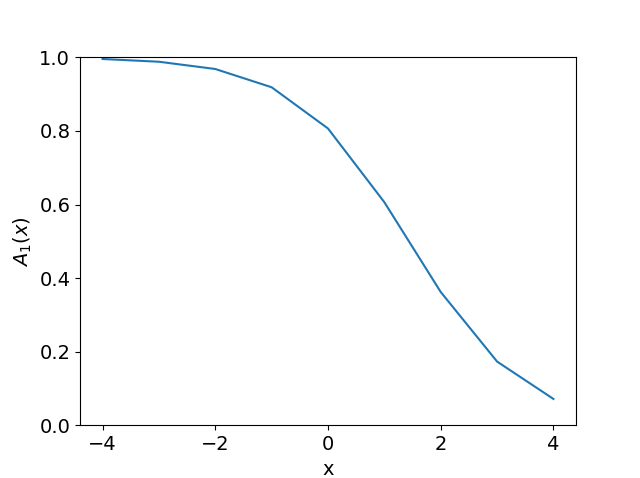
\includegraphics[width=0.5\textwidth]{img/pripadnostx-prvo-pravilo.png}}
    \subfloat{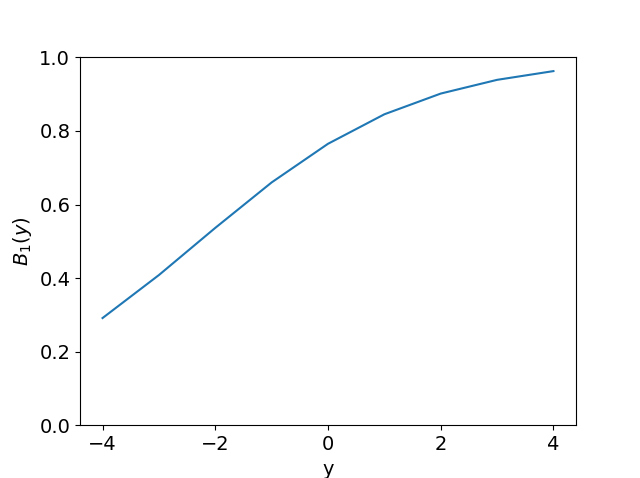
\includegraphics[width=0.5\textwidth]{img/pripadnosty-prvo-pravilo.png}}
    \caption{Funkcije pripadnosti za prvo pravilo}
\end{figure}
\begin{figure}[H]
    \subfloat{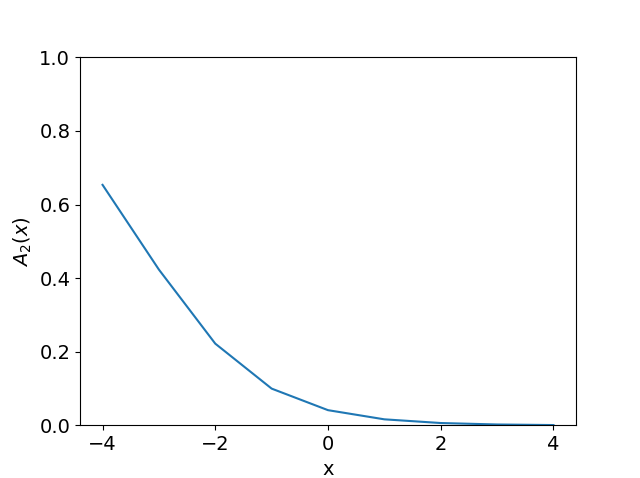
\includegraphics[width=0.5\textwidth]{img/pripadnostx-drugo-pravilo.png}}
    \subfloat{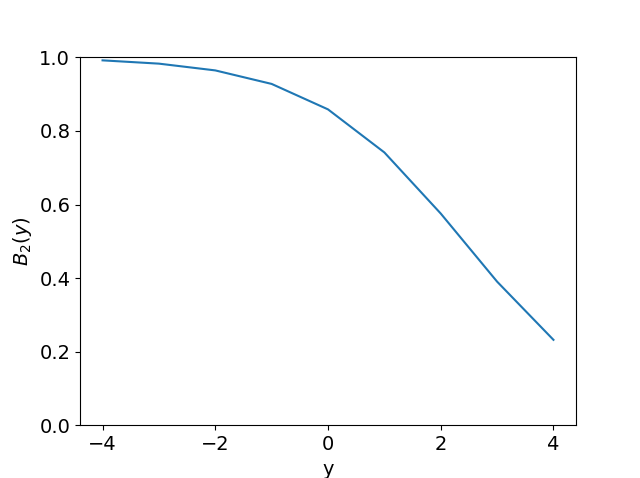
\includegraphics[width=0.5\textwidth]{img/pripadnosty-drugo-pravilo.png}}
    \caption{Funkcije pripadnosti za drugo pravilo}
\end{figure}
\begin{figure}[H]
    \subfloat{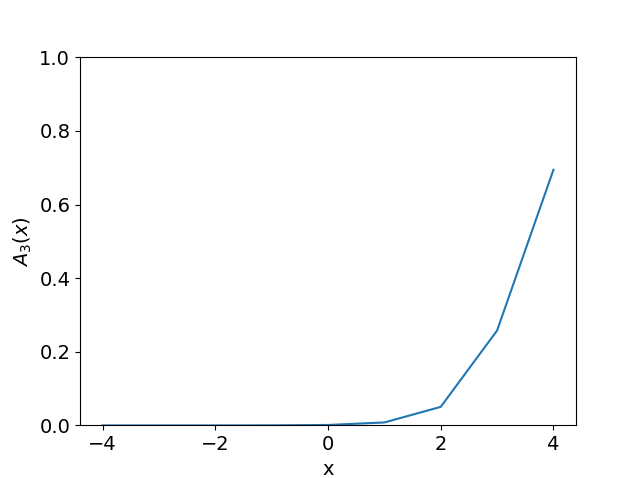
\includegraphics[width=0.5\textwidth]{img/pripadnostx-trece-pravilo.png}}
    \subfloat{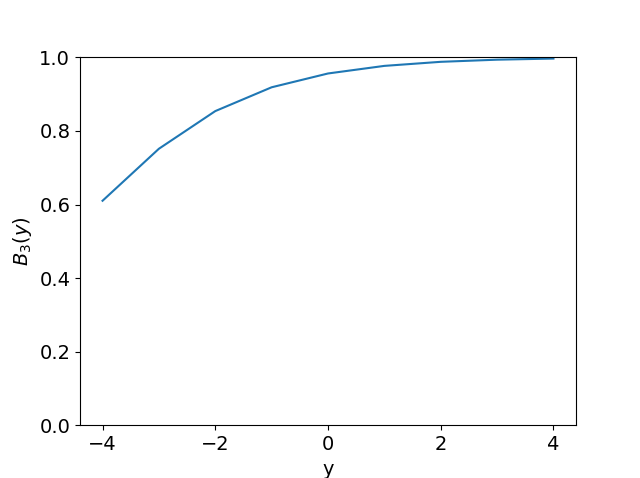
\includegraphics[width=0.5\textwidth]{img/pripadnosty-trece-pravilo.png}}
    \caption{Funkcije pripadnosti za treće pravilo}
\end{figure}
\begin{figure}[H]
    \subfloat{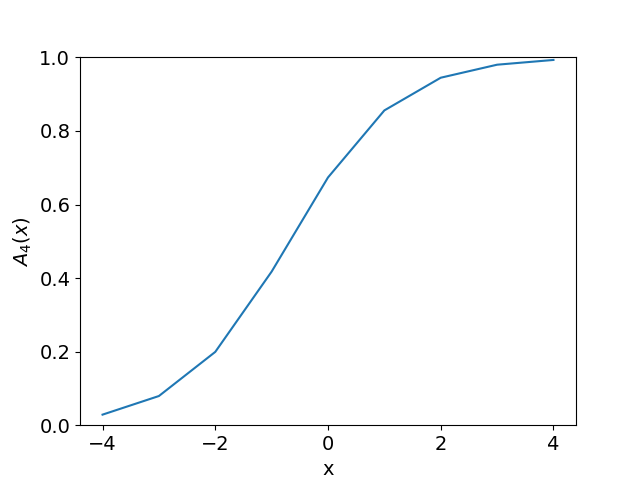
\includegraphics[width=0.5\textwidth]{img/pripadnostx-cetvrto-pravilo.png}}
    \subfloat{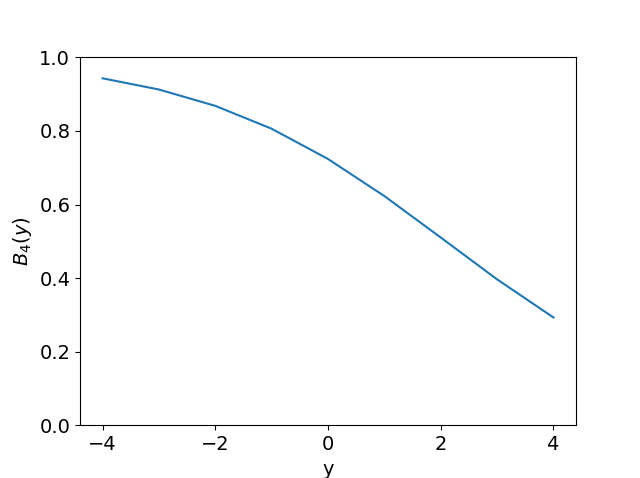
\includegraphics[width=0.5\textwidth]{img/pripadnosty-cetvrto-pravilo.png}}
    \caption{Funkcije pripadnosti za četvrto pravilo}
\end{figure}
\begin{figure}[H]
    \subfloat{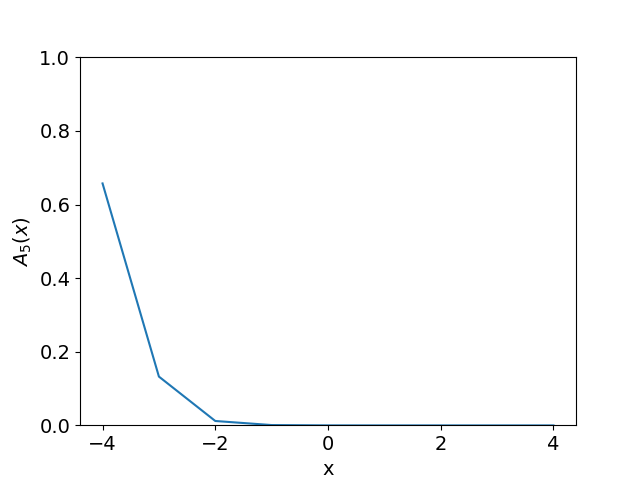
\includegraphics[width=0.5\textwidth]{img/pripadnostx-peto-pravilo.png}}
    \subfloat{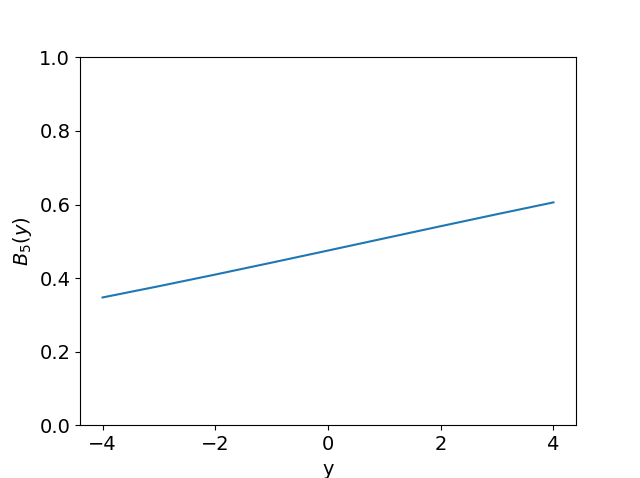
\includegraphics[width=0.5\textwidth]{img/pripadnosty-peto-pravilo.png}}
    \caption{Funkcije pripadnosti za peto pravilo}
\end{figure}
\begin{figure}[H]
    \subfloat{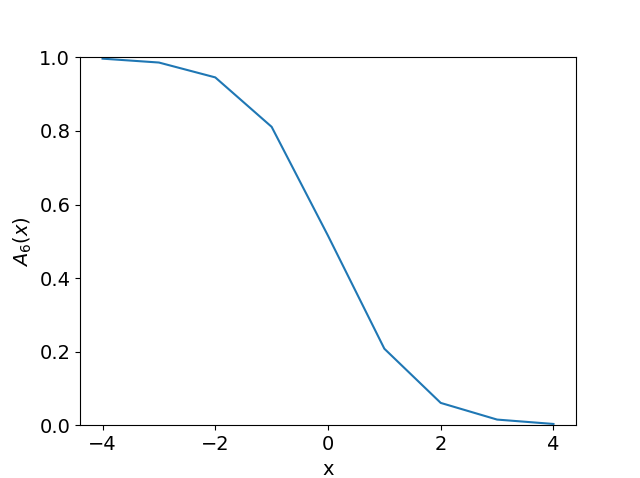
\includegraphics[width=0.5\textwidth]{img/pripadnostx-sesto-pravilo.png}}
    \subfloat{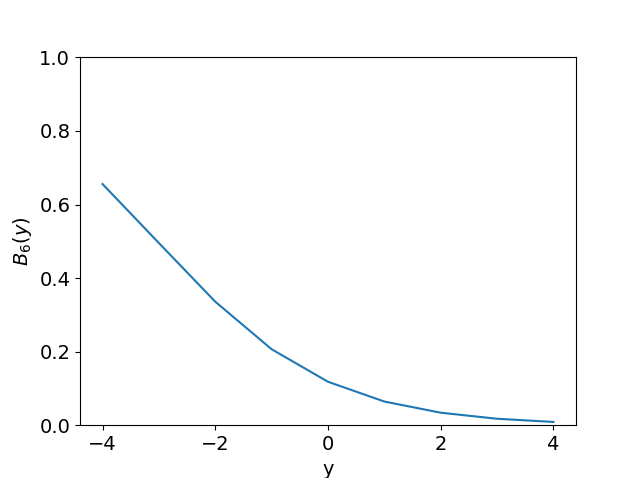
\includegraphics[width=0.5\textwidth]{img/pripadnosty-sesto-pravilo.png}}
    \caption{Funkcije pripadnosti za šesto pravilo}
\end{figure}
\begin{figure}[H]
    \subfloat{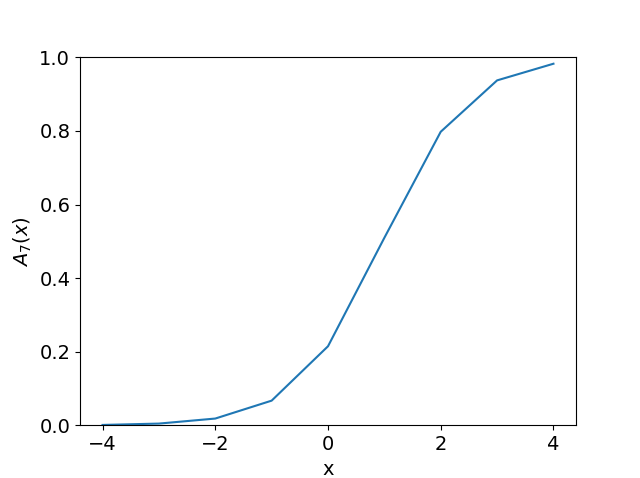
\includegraphics[width=0.5\textwidth]{img/pripadnostx-sedmo-pravilo.png}}
    \subfloat{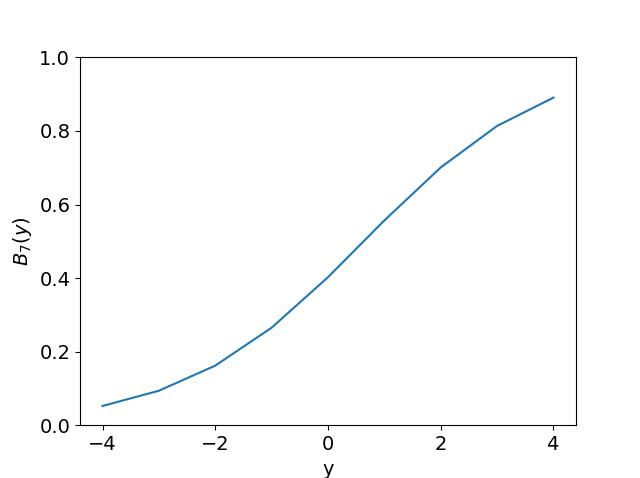
\includegraphics[width=0.5\textwidth]{img/pripadnosty-sedmo-pravilo.png}}
    \caption{Funkcije pripadnosti za sedmo pravilo}
\end{figure}

\chapter{Zadatak 7}
\begin{figure}[H]
    \centering
    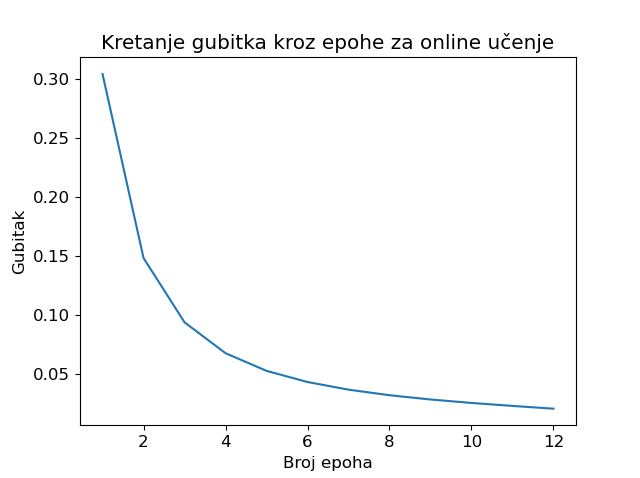
\includegraphics[scale=0.5]{img/loss-online.png}
    \caption{}
\end{figure}
\begin{figure}[H]
    \centering
    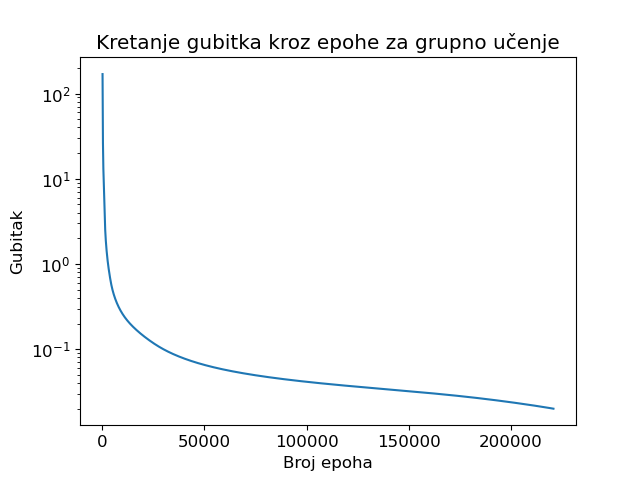
\includegraphics[scale=0.5]{img/loss-grupno.png}
    \caption{}
\end{figure}
Možemo vidjeti da \textit{online} učenje puno brže konvergira nego li grupno, no valja uzeti u obzir i stope učenja. U ovom eksperimentu za \textit{online} učenje su korištene stope učenja $10^{-3}$ i $3\cdot10^{-4}$, dok za grupno $10^{-4}$ i $3\cdot10^{-5}$. Dakle, razlika u redu veličina je 10.

\chapter{Zadatak 8}
\begin{figure}[H]
    \centering
    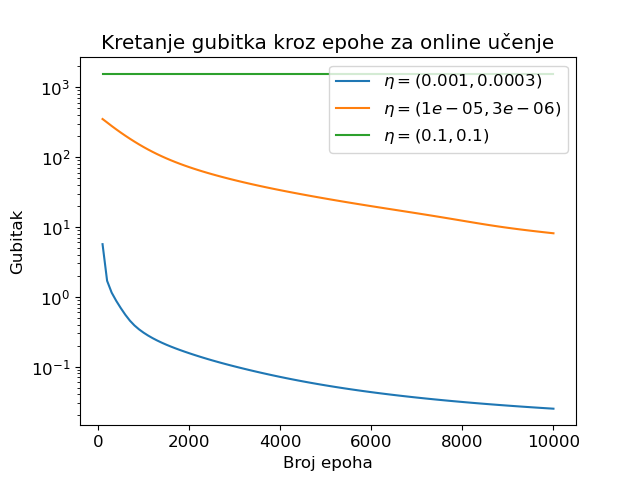
\includegraphics[scale=0.5]{img/stope-online.png}
    \caption{}
\end{figure}
\begin{figure}[H]
    \centering
    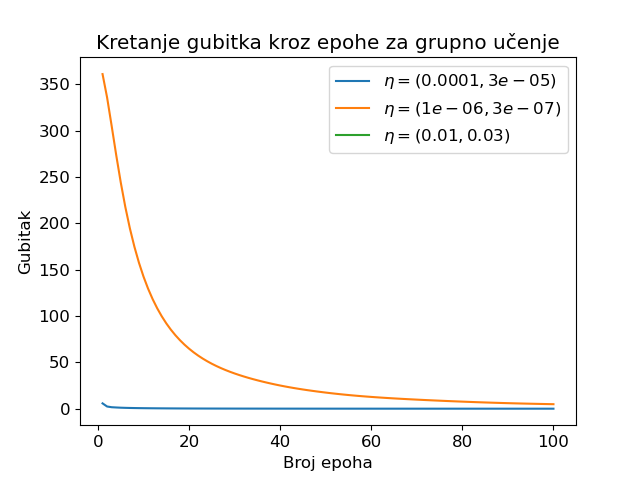
\includegraphics[scale=0.5]{img/stope-grupno.png}
    \caption{}
\end{figure}
Što je stopa učenja manja, to algoritam sporije konvergira, ali konvergira, dok što je stopa učenja veća, algoritam divergira. Također, optimalni iznosi stopa učenje za \textit{online} i grupno učenje razlikuju se za 10 puta.

\bibliography{literatura}
\bibliographystyle{fer}
\nocite{*}

\end{document}
